\documentclass[12pt]{article}
\usepackage{polski}
\usepackage[utf8]{inputenc}
\usepackage[T1]{fontenc}
\usepackage{times}

\usepackage{amsfonts}
\usepackage{amsmath}
\usepackage{bm}
\usepackage{mathtools}
\mathtoolsset{showonlyrefs}


\usepackage{tabularx}
\usepackage{array}
\newcolumntype{Y}{>{\centering\arraybackslash}X}
\newcolumntype{Z}{>{\centering\arraybackslash}p}
\usepackage{multirow}
\usepackage{hyperref}

\usepackage{enumitem}
\usepackage{float}


\usepackage{graphicx}
\usepackage{rotating}
\usepackage{subcaption}


\usepackage{animate}

\renewcommand{\thesection}{\arabic{section}}
\renewcommand{\thesubsection}{\arabic{section}.\arabic{subsection}}
\usepackage{wrapfig}



\usepackage{amsmath}
\usepackage{amsthm}
\usepackage{dsfont}
\newtheorem{lema}{Lemma}

\newtheoremstyle{exer}{20pt}{10pt}{}{0pt}{\bfseries}{.\\}{.5em}{}
\theoremstyle{exer}
\newtheorem{ex}{Ex}

%\usepackage[a4paper,total={6in,10in}]{geometry}
\usepackage[a4paper,total={7in,10in}]{geometry}
%\newtheoremstyle{style name}{space above}{space below}{body font}{indent amount}{head font}{head punct}{after head space}{head spec}


\begin{document}
	\begin{titlepage}
		\begin{center}
			
			\textbf{\Huge  Wykorzystanie poznanych metod dotyczących analizy zależności liniowej
				do wybranych danych rzeczywistych}
			
			\vspace{0.5cm}
			
			\vspace{1.5cm}
			
			\textbf{\LARGE Autorzy}\\
			\vspace{0.5cm}
			\large Kacper Budnik, 262286\\
			\large Maciej Karczewski, 262282\\
			
			
			\vfill
			
			\vspace{0.4cm}
			

			
			\vspace{0.8cm}
			Wydział Matematyki	
			\today
		\end{center}
	\end{titlepage}
	\tableofcontents
	\newpage
	
	\section{Wprowadzenie}
	Diamenty są krystalicznym węglem, najtwardszym znanym materiałem na Ziemi. Są one tworzone w głębi Ziemi, w wysokich temperaturach i ciśnieniach, a ich wydobycie wymaga specjalistycznej wiedzy i wielu lat doświadczenia. Diamenty są najcenniejszymi kamieniami szlachetnymi na świecie i są cenione zarówno przez osoby prywatne, jak i przez przemysł jubilerski. Blask i niezwykła trwałość diamentów sprawiają, że są one bardzo cenione, a ich cena zależy od wielu czynników, takich jak kolor, czystość, kształt i wielkość. Najcenniejsze diamenty są przezroczyste i bezbarwne, choć mogą też być innego koloru np.  żółte, niebieskie, czerwone czy zielone.
	
	Diamenty są często wykorzystywane do produkcji biżuterii. Są również używane  w  narzędziach do cięcia i szlifowania oraz w elektronice. W ostatnich latach diamenty zaczęły być również używane jako narzędzia do badań naukowych, ponieważ ich niezwykła trwałość i twardość sprawiają, że są one idealnymi materiałami do wielu zastosowań.
	
	Dane o diamentach pozyskujemy z platformy \href{https://www.kaggle.com}{Kaggle}. Nasze dane zawierają $53940$ rekordów i pierwsze $7$ wierszy wygląda następująco:
	\begin{table}[H]
		\resizebox{\textwidth}{!}{%
			\begin{tabular}{|l|l|l|l|l|l|l|l|l|l|l|}
				\hline
				& carat & cut & color & clarity & depth & table & price & x & y & z \\ \hline
				1 & 0.23 & Ideal & E & SI2 & 61.5 & 55 & 326 & 3.95 & 3.98 & 2.43 \\ \hline
				2 & 0.21 & Premium & E & SI1 & 59.8 & 61 & 326 & 3.89 & 3.84 & 2.31 \\ \hline
				3 & 0.23 & Good & E & VS1 & 56.9 & 65 & 327 & 4.05 & 4.07 & 2.31 \\ \hline
				4 & 0.29 & Premium & I & VS2 & 62.4 & 58 & 334 & 4.2 & 4.23 & 2.63 \\ \hline
				5 & 0.31 & Good & J & SI2 & 63.3 & 58 & 335 & 4.34 & 4.35 & 2.75 \\ \hline
				6 & 0.24 & Very Good & J & VVS2 & 62.8 & 57 & 336 & 3.94 & 3.96 & 2.48 \\ \hline
				7 & 0.24 & Very Good & I & VVS1 & 62.3 & 57 & 336 & 3.95 & 3.98 & 2.47 \\ \hline
			\end{tabular}%
		}
		\caption{Oryginalne dane.}
		\label{orginalne_dane}
	\end{table}
	

	\section{Przygotowanie danych do analizy}
	Analizowane dane obejmują okres od listopada 1996 roku, jednak w pierwszych latach dane były pobierane w różnych odstępach czasu. Dlatego rozpatrujemy dane z okresu od 1 stycznia 2008 do 31 grudnia 2015 roku, równo 8 lat. Pozostałe dane tj. pochodzące z okresu 1 styczeń 2016 -- 24 kwiecień 2017 pozostawiliśmy jako dane testowe. W tych okresach pomiary były robione 8 razy dziennie, co 3 godziny każdy, rzadkie przypadki pomiarów w dodatkowych porach zostały pominięte. Za obserwacje odstające uznaliśmy te, które spełniają poniższą własność
	\begin{equation}
		y\notin\left(Q_1-1.5IQR,Q_3+1.5IQR\right),
	\end{equation}
	gdzie $y$ jest kandydatem na obserwacje odstającą, $Q_1$ i $Q_3$ to odpowiednio pierwszy i trzeci kwantyl, a $IQR$ jest rozstępem międzykwantylowym. W wyniku tej obserwacji odrzuciliśmy jedynie 4 obserwacje rzędu 90$^\circ$C. Pozostałe wyniki należą do przedziału od 1$^\circ$C do 47$^\circ$C. Naszym celem jest analiza średniej dziennej temperatury, zatem w kolejnym kroku obliczyliśmy tą średnią. Jej wartości mieszą się w przedziale od 6$^\circ$C do 40$^\circ$C. Uzyskane średnie temperatury rzeczywiście były osiągane w Indiach w odpowiednich czasach.
	
	
	\section{Dekompozycja szeregu czasowego}
	\subsection{Wykresy dla surowych danych}
	Dekompozycję zaczniemy od analizy wykresów funkcji autokowariancji oraz częściowej autokowariancji. Prezentują się one następująco
	\begin{figure}[H]\label{fig:dry_cov}
		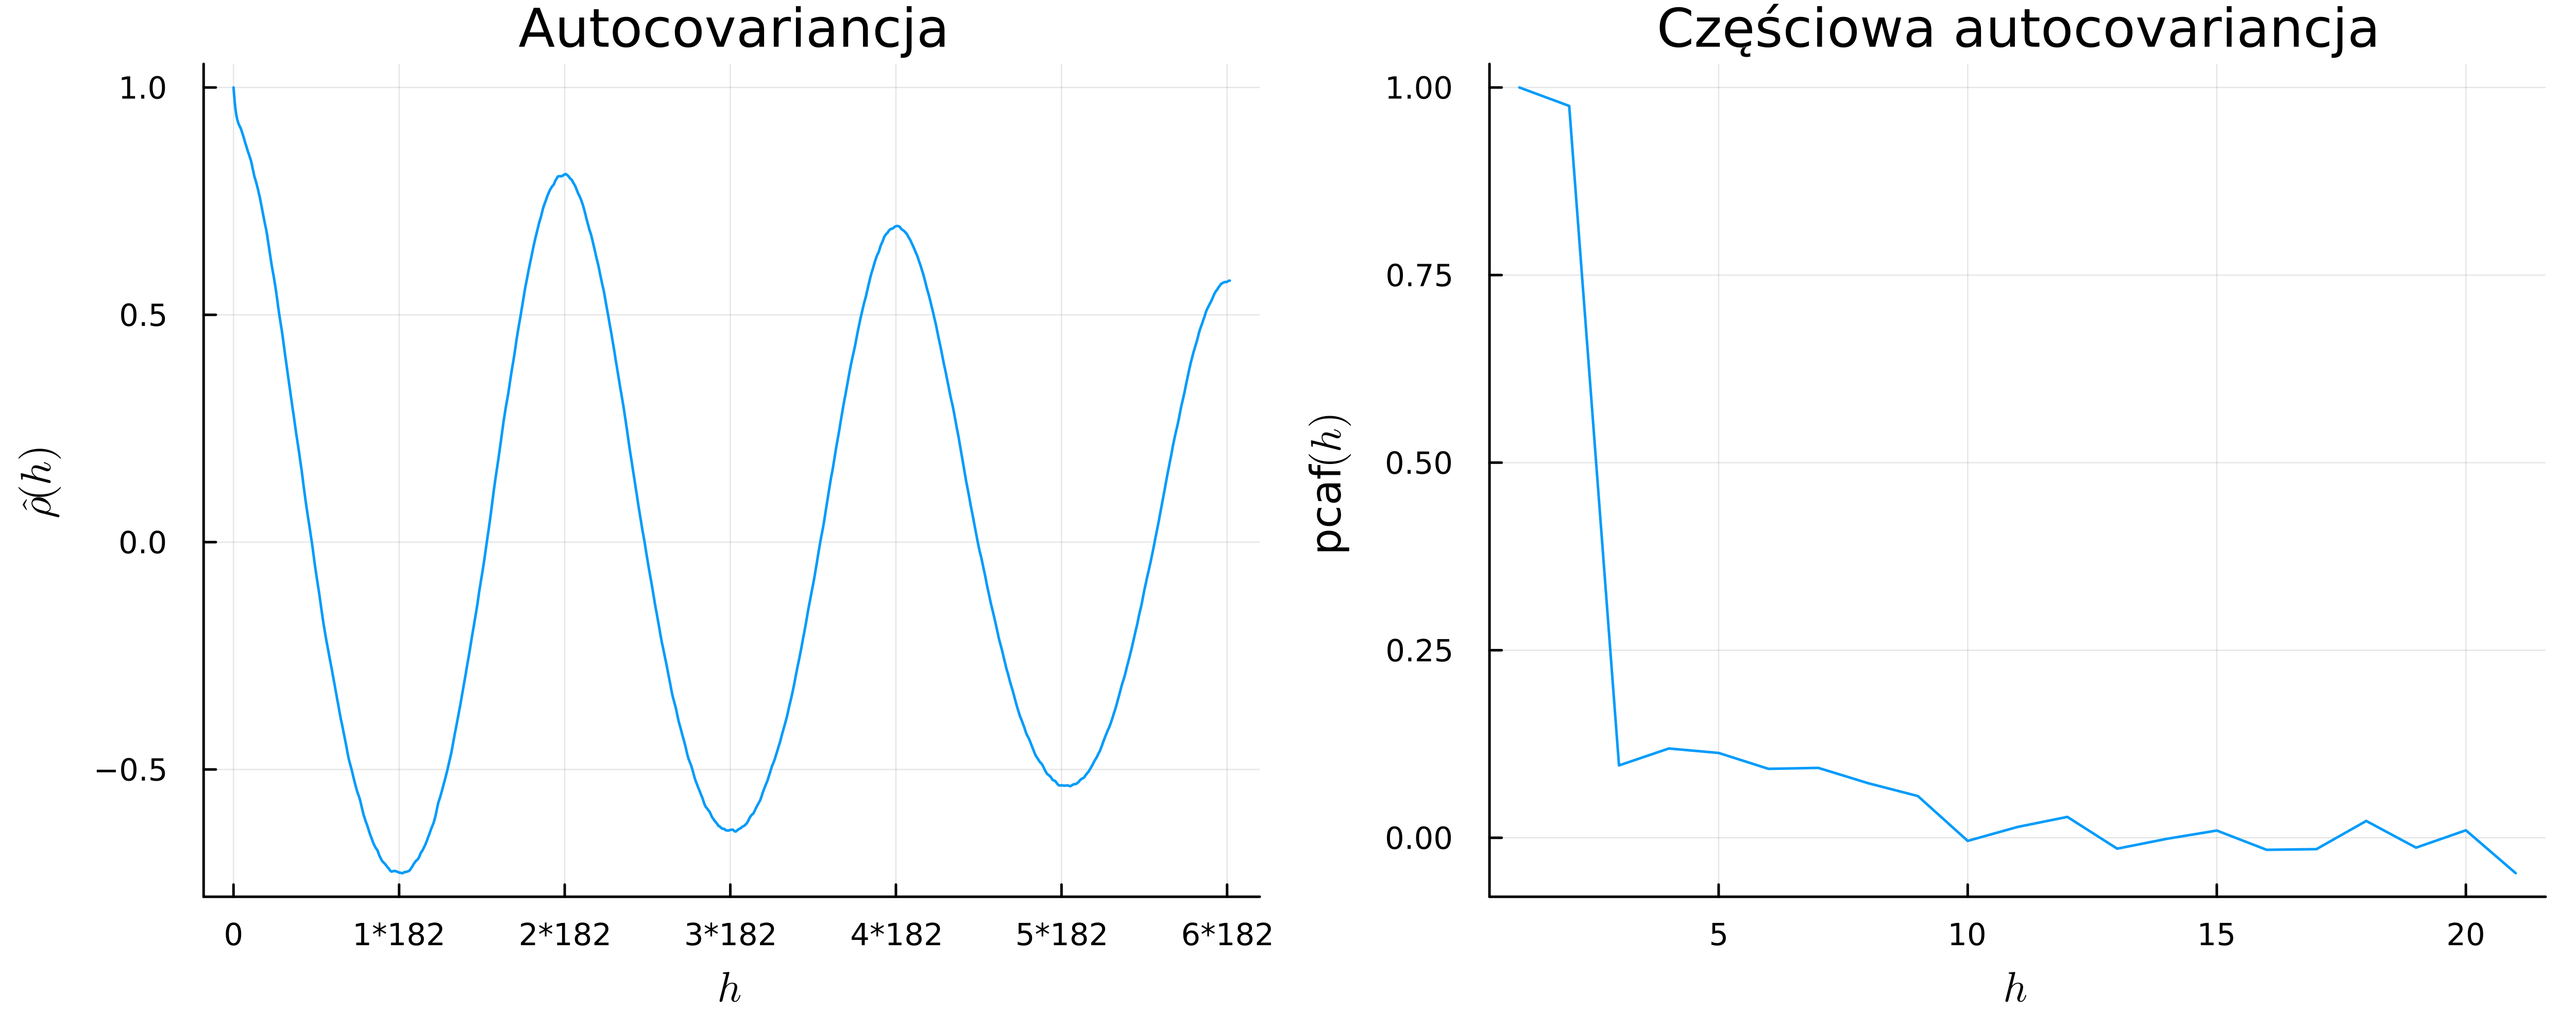
\includegraphics[width=\columnwidth]{Budnik/img/auto_dry.png}
		\caption{Funkcjie empircznej autokowariancji i częściowej autokowariancji.}
	\end{figure}
	Na powyższym wykresie widać okresowe zachowanie funkcji autokowariancji z okresem około 365. Liczba ta pokrywa się z liczbą dni w roku, co wydaje się intuicyjne. Z powodu na globalne ocieplenie możemy podejrzewać, że będzie istniał dodatni trend. Rzeczywiście, korzystając z funkcji \verb*|polyfit|, otrzymaliśmy trend
	\begin{equation}
		m(h)=24.8564+9\cdot10^{-5}h,
	\end{equation}  
	gdzie $m$ oznacza zmianę średniej temperatury w ciągu dnia. Zatem w ciągu 10 lat średnia temperatura w Delhi, według naszych obliczeń, wzrosła w przybliżeniu o $m(10\cdot365)-m(0)\approx0.3287^\circ$C. Według danych w tym samym okresie średnia temperatura na ziemi wzrosła, w zależności od regionu i źródeł, o więcej niż $0.2^\circ$C, zatem nasze wyniki częściowo pokrywają się z obserwowanymi zdarzeniami.
	\subsection{Transformacja Boxa-Coxa}
	Przed przystąpieniem do dekompozycji zastosowaliśmy transformację Boxa-Coxa. Transformacja ma ta na celu zminimalizowanie wariancji i przybliżenie rozkładu do rozkładku normalnego. Przy pomocy metod numerycznych oszacowaliśmy, że najmniejsza wariancja będzie dla transformacji z parametrem $\lambda\approx1.4591$, zatem analizować dane w postaci $y_n=x_n^\lambda$. Na poniższym histogramie widnieją dane przed transformacją (niebieski) oraz po transformacji (pomarańczowy).
	\begin{figure}[H]
		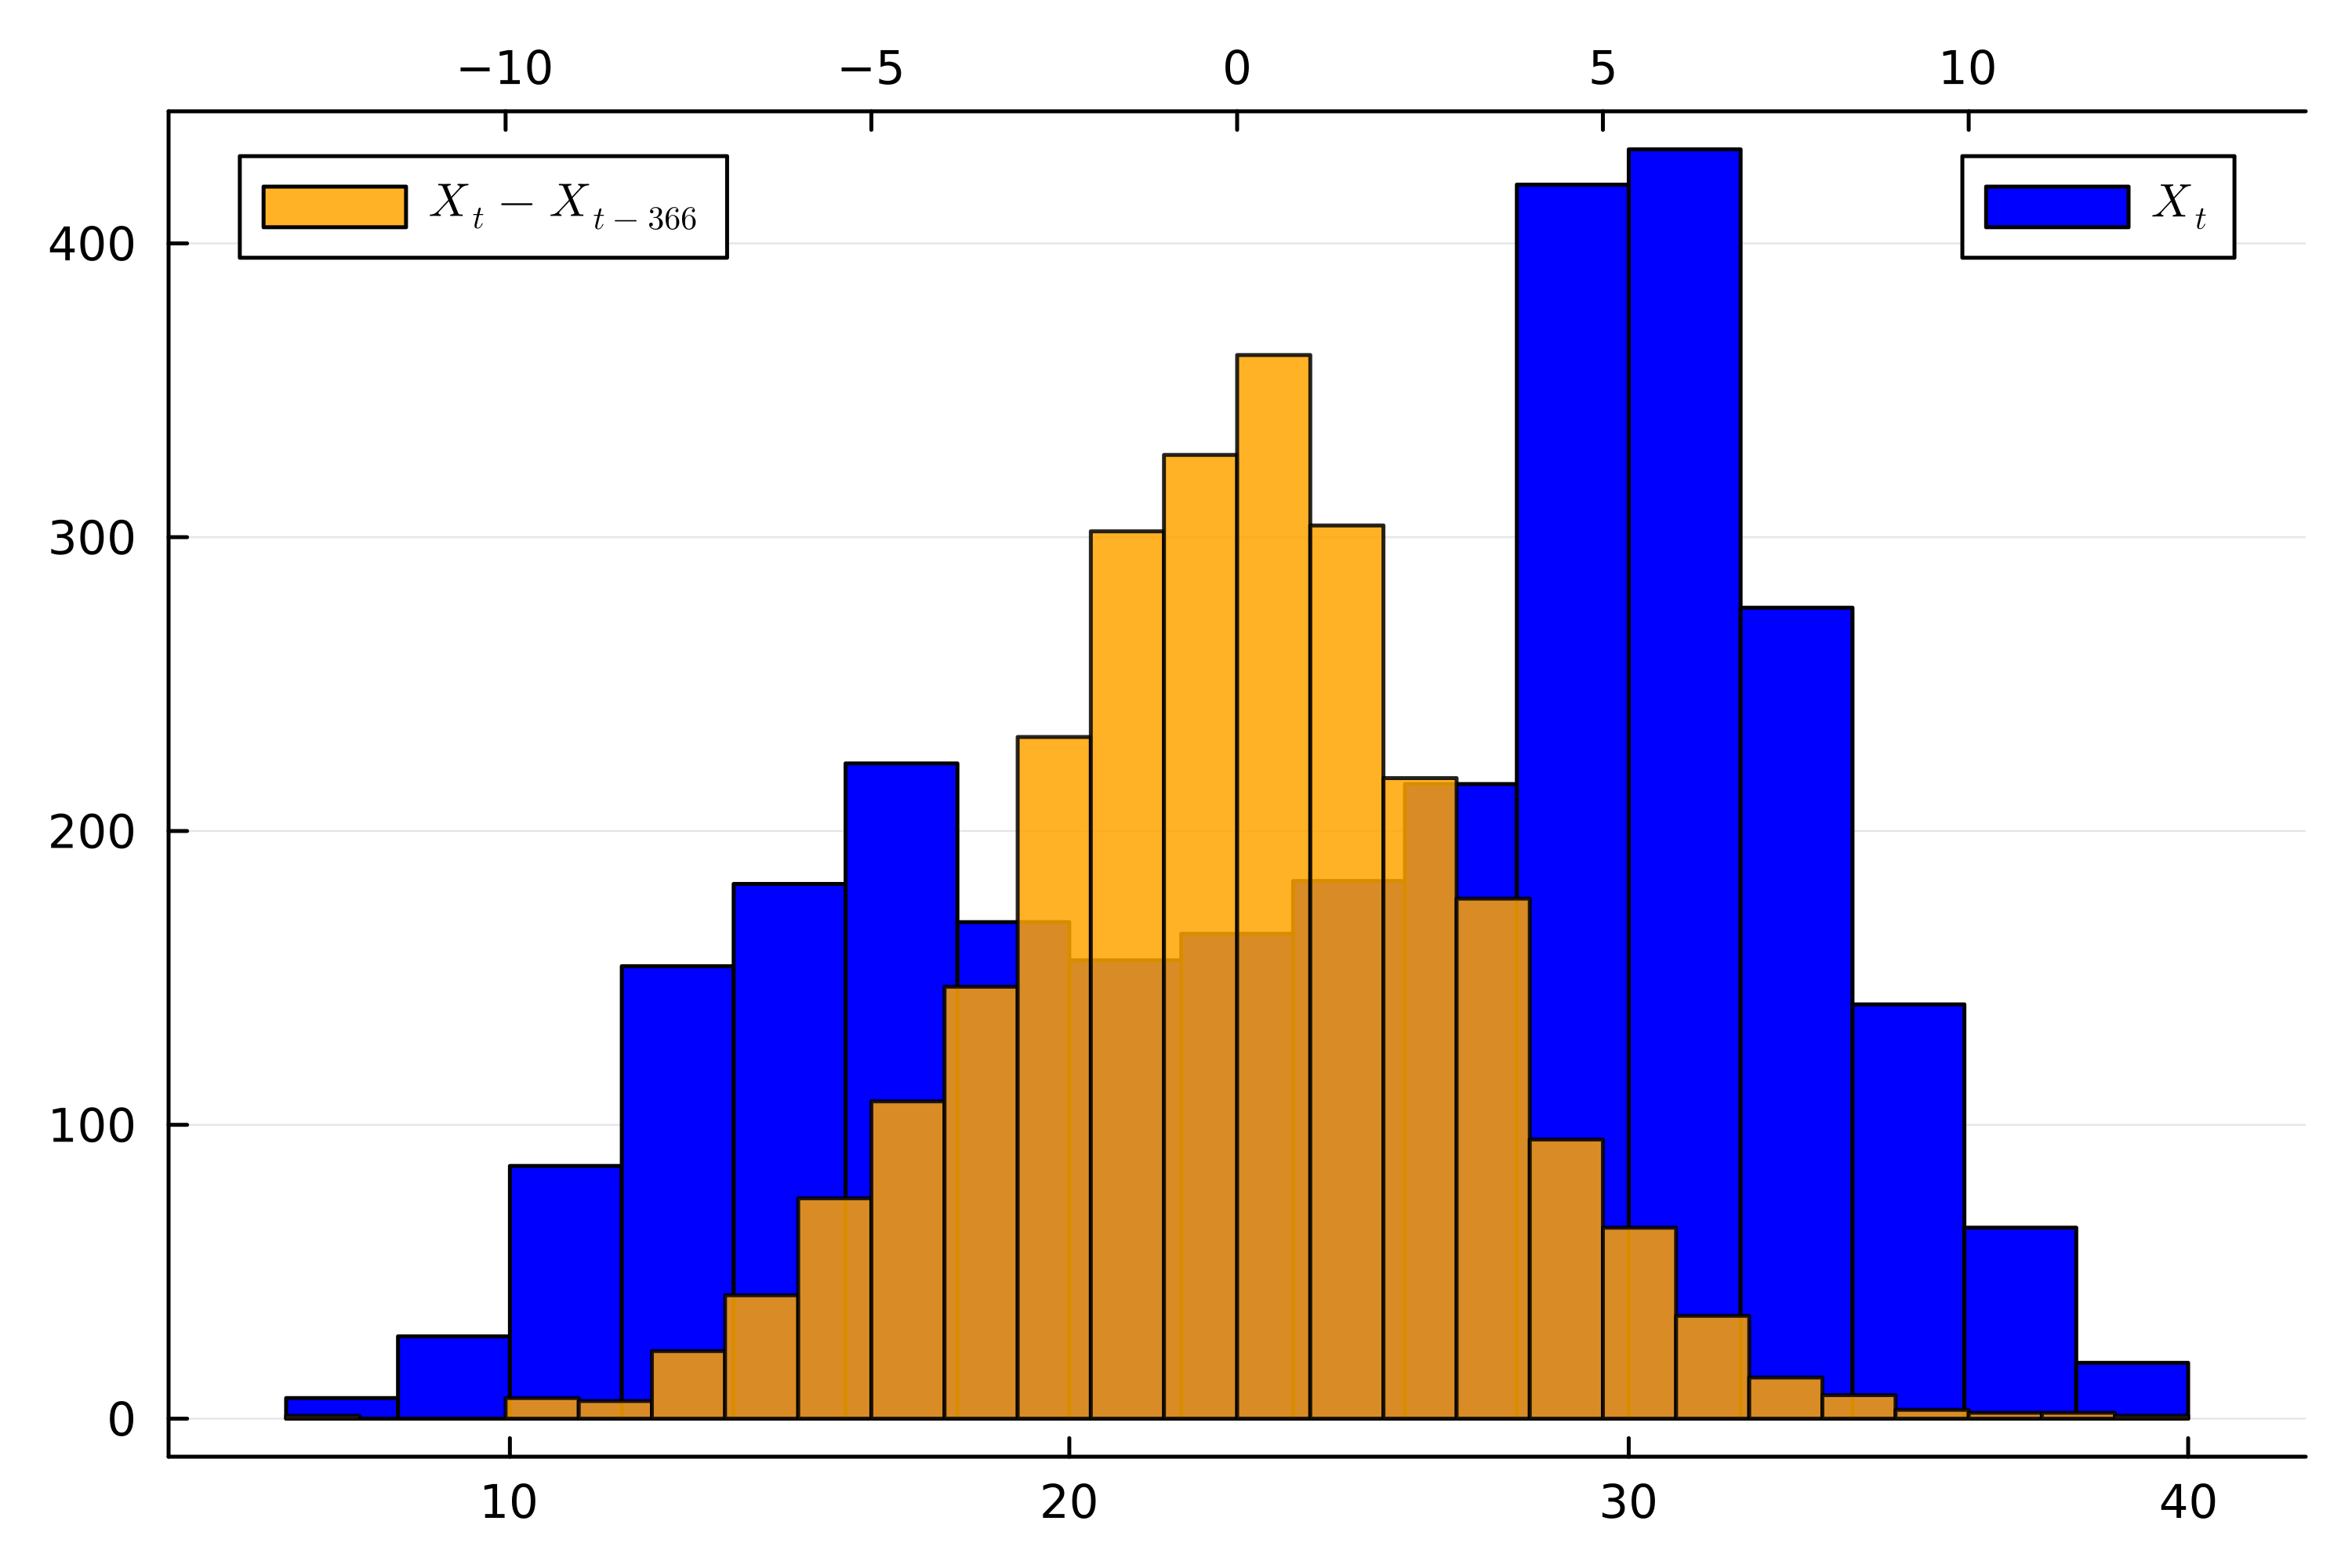
\includegraphics[width=\columnwidth]{Budnik/img/BoxCox.png}
		\caption{Dane przed i po transformacji. Dolna oś wskazuje na dane oryginalne, na górze widnieje oś dla danych po transformacji.}
	\end{figure}
	\subsection{Różnicowanie sezonowe}
	Tak jak już wspomnieliśmy, przy analizie wykresu \autoref{fig:dry_cov}, nasze dane wykazują okresowość z okresem 365 dni. By pozbyć się tych sezonowości zastosowaliśm różnicowanie sezonowe, czyli analizowaliśmy dalej dane w postaci
	\begin{equation}
		W_t=Y_t-Y_{t-360}.
	\end{equation}
	
	
	\section{Jednowymiarowa analiza}
	\subsection{Objętość}
	Analizę danych zaczniemy od analizy objętości. Box plot objętości wygląda następująco.

	Jak możemy zobaczyć na box plocie nasze dane mają dużo wartość odstających. Z tego powodu ciężko analizować wykres \ref{fig:box_V_orginal}, a także stworzyć poprawny model, dlatego pozbędziemy się ich. Po usunięciu obserwacji odstających otrzymamy czytelniejszy wykres.

	Tutaj nasze dane są o wiele bardziej czytelne. Z wykresu \ref{fig:box_V} możemy odczytać, że mediana naszych danych wynosi około $95$ oraz, że mamy do czynienia z rozkładem prawostronnie skośnym. Widzimy też, że pierwszy kwantyl wynosi około $60$ a trzeci około $160$.
	Zobaczymy teraz jak wygląda rozkład objętości na histogramie.

	Jak widzimy na histogramie gęstość nie zachowuje się monotoniczne, ciężko stwierdzić jaki rozkład ma objętość. Pomimo tego faktu możemy zauważyć, że diamenty dzielą się głównie na $4$ grupy. Pierwszą, najliczniejszą, jest grupa o iloczynie wymiarów należących do przedziału $[45;70] $, następną jest grupa o iloczynie należącym do $[80;100]$. Pozostałymi grupami są iloczyny należące do przedziałów $[110;120]$ oraz $[160;170]$.
	
	Zobaczymy teraz jak wyglądają statystyki opisowe dla naszych oczyszczonych danych.
	
	\begin{table}[H]
		\resizebox{\textwidth}{!}{%
			\begin{tabular}{|l|l|l|l|l|l|}
				\hline
				& Średnia & Mediana & Wariancja & Skośność & Kurtoza \\ \hline
				V & $113.48$ & $100.87$ & $3057.10$ & $0.60$ & $-0.63$ \\ \hline
			\end{tabular}%
		}
		\caption{Podstawowe statystyki opisowe dla objętości.}
		\label{tab:statystyki_V}
	\end{table}
	Możemy zobaczyć, że średnia jest większa  od mediany, oraz że skośność jest dodatnia co sugeruje nam, że rozkład objętości jest prawostronnie skośny, co się pokrywa za informacją zawartą na box plocie \ref{fig:box_V}. Kurtoza jest ujemna to znaczy, że rozkład ma ogony węższe niż rozkład normalny czyli jest rozkładem platykurtycznym. 
	
	\subsection{Cena}
	Sprawdziliśmy jak wygląda rozkład objętości to teraz sprawdzimy rozkład ceny diamentów.
	Box Plot dla ceny diamentów bez usunięcia wartości skrajnych wygląda następująco.
	
	Z box plotu możemy odczytać, że ponownie mamy dużo wartości odstających, które przeszkadzają w analizie danych. Właśnie z tego powodu usuniemy $ 1 \% $ najmniejszych cen oraz  $ 10\%$ największych cen.
	Po usunięciu wartości nasz Box plot wygląda następująco

	Po usunięciu danych skrajnych wykres pudełkowy staje się czytelniejszy. Z wykresu możemy odczytać, że mediana cen jest w okolicy $2000$, natomiast pierwszy w okolicach $1000$, a trzeci w okolicach $4300$. Możemy sądzić, że rozkład ceny jest prawostronnie skośny.
	

 Z histogramu możemy odczytać, że gęstość prawdopodobieństwa ceny jest prawie monotoniczna. Im większa cena tym na ogół, rzadszy diament. Możemy zobaczyć, że mamy najwięcej diamentów tanich nieprzekraczających $2500$ . Możemy także zobaczyć większą liczebność diamentów z ceną w okolicach $4000$. 
 
		Zobaczymy teraz jak wyglądają statystyki opisowe dla naszych oczyszczonych danych
	
	\begin{table}[H]
		\resizebox{\textwidth}{!}{%
			\begin{tabular}{|l|l|l|l|l|l|}
				\hline
				& Średnia & Mediana & Wariancja & Skośność & Kurtoza \\ \hline
				Cena &$2890.46$ & $2064.0$ 	 & $5.49 \cdot 10^6 $ & $1.02$  &$0.10$ \\ \hline
			\end{tabular}%
		}
		\caption{Podstawowe statystyki opisowe dla objętości.}
		\label{tab:statystyki_price}
	\end{table}
	Możemy zobaczyć, że średnia jest większa od mediany, oraz że skośność jest dodatnia co sugeruje nam, że rozkład objętości jest prawostronnie skośny co się pokrywa za informacją zawartą na box plocie \ref{fig:box_price}. Kurtoza jest dodatnia, ale bliska $0$ to znaczy, że rozkład ma ogony grubsze niż rozkład normalny lub ma porównywalne do rozkładu normalnego. Zatem jest to rozkład leptokurtyczny lub mezokurtyczny. Wariancja ceny jest znacząco większa niż wariancja obiętości w tabeli\ref{tab:statystyki_V}.  
	
	\section{Analiza zależności między między ceną, a objętością diamentu}
	Po omówieniu danych oraz ich wstępnym przetworzeniu, możemy przystąpić do analizy. Celem naszym będzie przeanalizować zależność między ceną, a objętością oraz dopasowanie krzywej regresji. Zanim rozpoczniemy analizę, w celu określenia rodzaju zależności, przyjrzyjmy się wykresowi zależności między danymi. %Zanim rozpoczniemy analizę, przyjrzyjmy się ich zależności na wykresie.

	\noindent Na wykresie możemy zauważyć silną zależność między naszymi danymi. Z powodu rozłożenia naszych danych, zależność ta może być liniowa. W celu określenia tej zależności obliczymy podstawowe statystyki
	\begin{itemize}
		\item $SST=\sum_{i=1}^n(y_i-\overline{y})^2\approx1.409e11$,
		\item $SSE=\sum_{i=1}^n(\hat y_i-y_i)^2\approx2.015e10$,
		\item $SSR=\sum_{i=1}^n(\hat y_i-\overline{y})^2\approx1.207e11$,
	\end{itemize}
	oraz, najbardziej nas interesujący, współczynnik korelacji Pearsona
	\begin{equation}
		\rho=\frac{\sum_{i=1}^n\left(x_i-\overline{x}\right)\left(y_i-\overline{y}\right)}
		{\sqrt{\sum_{i=1}^n\left(x_i-\overline{x}\right)^2}\sqrt{\sum_{i=1}^n\left(y_i-\overline{y}\right)^2}}\approx0.93,
	\end{equation}
	gdzie $x_i$, $y_i$ to $i$-te obserwacje odpowiednio objętości oraz ceny, $\overline{x}$ oznacza średnią z $x$, a $n$ to rozmiar próby, oznaczeniami tymi będziemy posługiwali się w całym raporcie. Wartość ta jest blisko wartości $1$, zatem nasze dane są silnie skorelowane dodatnie oraz liniowo. Dodatkowo wartości $SST$ oraz $SSR$ są relatywnie blisko siebie, a suma błędów $SSE$ jest rząd mniejsza od pozostałych. W tym przypadku regresja liniowa powinna być odpowiednim wyborem. Dlatego, model którym będziemy opisywać dane będzie miał postać
	\begin{equation}\label{eq:reg}
		Y_i=\beta_0+\beta_1x_i+\xi_i,
	\end{equation}
	gdzie $\xi_i$ jest losowym błędem pomiarowym. $Y_i$ jest zmienną losową, której realizacją jest zaobserwowana wartość $y_i$. Zgodnie z wytycznymi dotyczących naszego zadania, zakładamy, że wszystkie zminne losowe $\xi_i$ są iid. o rozkładzie normalny ze średnią 0. Naszym celem będzie estymować wartość $\hat y_i$ poprzez estymowanie realizacji zmiennych losowych $\hat \beta_0$ oraz $\hat\beta_1$.
	\subsection{Estymacja punktowa}
	By stworzyć estymator ceny $\hat y$ skorzystamy z metody najmniejszych kwadratów. Do estymacji parametrów $\beta_0$ oraz $\beta_1$, występujące we wzorze \eqref{eq:reg}, wykorzystamy losowo wybrane $80\%$ naszych danych. Pozostałe $20\%$ posłuży nam w celu sprawdzenie poprawności modelu. Dane zostały wylosowane przy użyciu podstawowych funkcji języka \verb|Julia| z ustalonym ziarnem. Estymowane parametry, w zaobserwowanej realizacji $Y=(Y_1, Y_2,\cdots,Y_n)$, mają wartość
	\begin{equation}
		\hat\beta_1=\frac{\sum_{i=1}^n\left(x_i-\overline{x}\right)\left(y_i-\overline{y}\right)}
		{\sum_{i=1}^n\left(x_i-\overline{x}\right)^2}\approx39.089 \quad \text{oraz} \quad
		\hat\beta_0=\overline{y}-\beta_1\overline{x}\approx-1548.34\ .
	\end{equation}
	Zatem estymowana wartośc ceny $\hat y$ modelu \eqref{eq:reg} będzie miała postać
	\begin{equation}\label{eq:model}
		\hat y_i = 38.089\cdot x_i -1548.34\ .
	\end{equation}
	\subsection{Estymacja przedziałowa}
	W tym przypadku będziemy szukać przedziału, w którym będzie należał nasz $Y_i$ z dużym prawdopodobieństwem. Będziemy chcieli by prowdopodobieństow to wynosiło $1-\alpha$. Znany jest fakt, że w modelu \eqref{eq:reg} zmienna $\hat{Y}_i$ ma poniższe parametry
	\begin{equation}
		\mathbb{E}\hat Y_i = \beta_0+\beta_1x_i \quad\text{oraz}\quad Var \hat Y_i=Var\left(\xi_1\right)\left(\frac{1}{n}+\frac{(x_0-\overline{x})}{\sum_{i=1}^{n}\left(x_i-\overline{x}\right)^2}\right).
	\end{equation} 
	Jeśli $Var\left(\xi_1\right)$ nie jest znana w jej miejsce wstawiamy jej estymator
	\begin{equation}
		s^2=\frac{1}{n-2}\sum_{i=1}^{n}\left(Y_i-\hat Y_i\right)
	\end{equation}
	otrzymując estymator $Var \hat Y_i$. W tym przypadku zmienna losowa
	\begin{equation}
		\frac{\hat Y_i-\mathbb{E}\hat Y_i}{\sqrt{s^2\left(\frac{1}{n}+\frac{(x_0-\overline{x})}{\sum_{i=1}^{n}\left(x_i-\overline{x}\right)^2}\right)}}
	\end{equation}
	ma rozkład t-studenta z $n-2$ stopniami swobody. Przez $z_{\alpha/2}$ będziemy oznaczać $1-\alpha/2$ kwantyl z właśnie tego rozkładu. Dla estymowane wartość $\hat Y_0$, dla znanej objętości, równej $x_0$ będzie zachodziła równość
	\begin{equation}
		\mathbb{P}\left(\hat Y_0 - z_{\alpha/2}s\sqrt{\frac{1}{n}+\frac{\left(x_0-\overline{x}\right)^2}{\sum_{i=1}^n\left(x_i-\overline{x}\right)^2}}\leq Y_0\leq\hat Y_0 + z_{\alpha/2}s\sqrt{\frac{1}{n}+\frac{\left(x_0-\overline{x}\right)^2}{\sum_{i=1}^n\left(x_i-\overline{x}\right)^2}}\right)=1-\alpha.
	\end{equation}

	\noindent Zatem naszym przedziałem ufności ceny dla objętości $x_0$, w zaobserwowanej próbie, będzie przedział
	\begin{equation}\label{eq:ufność}
		\left(\hat y_0 - 	z_{\alpha/2}s\sqrt{\frac{1}{n}+\frac{\left(x_0-\overline{x}\right)^2}{\sum_{i=1}^n\left(x_i-\overline{x}\right)^2}}, \hat y_0 + z_{\alpha/2}s\sqrt{\frac{1}{n}+\frac{\left(x_0-\overline{x}\right)^2}{\sum_{i=1}^n\left(x_i-\overline{x}\right)^2}}\right).
	\end{equation}
     
     \subsection{Predykcja danych}
     Tak jak wspominaliśmy, $ 20\% $ danych posłuży nam do sprawdzenia modelu. Dla tych danych przyjrzymy się wartością rzeczywistym, estymowanym punktowo oraz przedziałowo.
     

Analizując wykres możemy zauważyć, że dane są w oklicach prostej regresyjnej \eqref{eq:model} dla małych obiętości. Wraz ze wzrostem iloczynu wymiarów rośnie też odległość danych od prostej. Do podobnych wniosków możemy dojść analizując przedziały ufności \eqref{eq:ufność} dla naszych danych. Fakt ten może sugerować nam, że objętość nie wpływa liniowo na cenę diamentu lub, że założenia dotyczące modelu nie okazały się poprawne.
%, w szczególności cena większych diamentów  nie jest liniowa od iloczynu wymiarów diamentu. 
Na poprawność regresji może wpływać również fakt, że diamenty mają jeszcze inne cechy, których nie bierzemy pod uwagę.
%Może wpływać na to fakt, że diamenty mają jeszcze inne cechy, których tutaj nie bierzemy pod uwagę. 
 \section{Analiza residuów}
 	Podczas tworzenia modelu regresji liniowej oraz dalszych obliczeń zakładaliśmy następujące warunki
 	\begin{enumerate}
 		\item $\mathbb{E}\xi_i=0$ $\forall i$ ,
 		\item $Var\xi_i=\sigma^2<\infty\quad\forall i$,
 		\item $\xi_i$ mają rozkład normalny,
 		\item $\xi_i\perp\!\!\!\perp\xi_j$ dla $i\neq j$.
 	\end{enumerate}
 	Do sprawdzienia tych warunków wykonamy analizę residuów $e_i$ danych wzorem
 	\begin{equation}
 		e_i=y_i-\hat y_i
 	\end{equation}
    Zaczniemy od sprawdzenia średniej rozkładu. W naszej próbie wynosi
	\begin{equation}
		\mathbb{E}\xi_i\approx\overline{e}=1.18e-8,
	\end{equation}
	zatem średnia residuów jest równa zeru, co nie jest zaskakujące, uwzględniając, że skorzystaliśmy z metody najmniejszych kwadratów. Przeanalizujmy jeszcze wykres residuów na poniższym wykresie.
	
	Na wykresie wyraźnie widać, że dla małych objętości wszystkie residua są znacznie większe od zera, więc ich wartość oczekiwana nie może być bliska zeru. Dodatkowo możemy zauważyć, że wraz ze zwiększającą się objętością, zwiększa się wariancja. Zatem pierwsze, jak i drugie założenie, nie jest spełnione. Do sprawdzenia założenia trzeciego o normalności rozkładu sprawdzimy wykorzystując histogram residuów.
	
	Na wykresie widzimy, że histogram nie pokrywa się z gęstością teoretyczną. Przed odrzuceniem założenia trzeciego, porównajmy jeszcze dystrybuantę naszych residuów oraz rozkładu normalnego oraz oba rozkłady na qqplocie.

	Również na tych wykresach widzimy znaczną różnicę między rozpatrywanymi rozkładami. Możemy więc z pewnością stwierdzić, że rozkład residuów nie jest normalny. Do sprawdzenia pozostaje nam założenie o niezależności błędu. W tym celu sprawdzimy, czy nasze zmienne są skorelowane.
	Wartości w estymatora autokowariancji nie są zerowe na prawo od początku układu współrzędnych, więc nasze residua są skorelowane. Dlatego możemy wywnioskować, że nasze dane są zależne, zatem czwarte założenie również musimy odrzucić.
	
	\section{Wnioski autorów}
	Początkowo wydawało się, że to model liniowy jednej zmiennej może dobrze estymować cenę. Niestety wynik końcowy zaprzeczył temu. Pomimo nawet współczynnika korelacji Pearsona bliskiego wartości 1.\\
	Możemy wywnioskować stąd, że cena diamentów nie zależy liniowo od ich objętości, ale ma ona znaczący wpływ na ich wartość, w szczególności dla małych rozmiarów. Wraz z rozmiarem rosła wariancja drogocennego kruszcu, a cena była rozłożona bardziej nieprzewidywalnie. Naszą hipotezą jest, że planując zakup diamentu o małej cenie, głównym kryterium będzie jego rozmiar. Jeśli nasz budżet na zakup jest większy, rozmiar schodzi na kolejny plan, ustępując miejsca innym własnością, takim jak na przykład przejrzystość, kolor, czy doskonałość cięcia.
	

\end{document}